\section{Box Model: Margin, Padding, dan Border}

Box model adalah konsep paling fundamental dalam CSS layout. Setiap elemen HTML divisualisasikan oleh browser sebagai sebuah \textbf{kotak} (box) yang terdiri dari empat lapisan konsentris: \textbf{content} (isi), \textbf{padding} (ruang dalam), \textbf{border} (garis batas), dan \textbf{margin} (ruang luar). Memahami box model adalah kunci untuk mengendalikan ukuran, spasi, dan posisi elemen di halaman web. Tanpa pemahaman ini, layout CSS akan terasa membingungkan dan tidak dapat diprediksi \cite{webdevCss}.

\begin{figure}[htbp]
\centering
\resizebox{0.75\textwidth}{!}{%
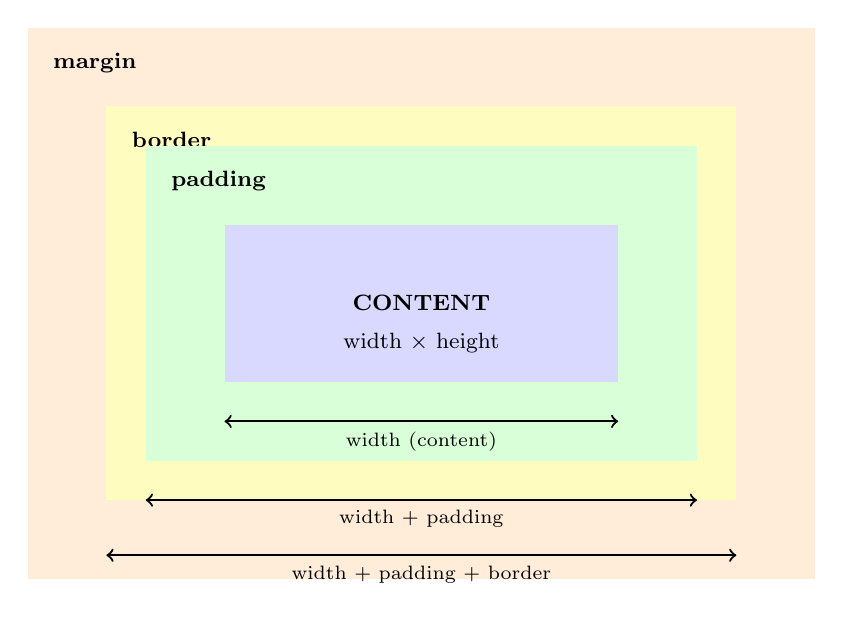
\begin{tikzpicture}[every node/.style={font=\footnotesize}]
  % Margin (outermost)
  \fill[orange!15] (0,0) rectangle (10,7);
  \node[anchor=north west] at (0.2,6.8) {\textbf{margin}};

  % Border
  \fill[yellow!25] (1,1) rectangle (9,6);
  \node[anchor=north west] at (1.2,5.8) {\textbf{border}};

  % Padding
  \fill[green!15] (1.5,1.5) rectangle (8.5,5.5);
  \node[anchor=north west] at (1.7,5.3) {\textbf{padding}};

  % Content
  \fill[blue!15] (2.5,2.5) rectangle (7.5,4.5);
  \node at (5,3.5) {\textbf{CONTENT}};
  \node at (5,3) {\code{width} $\times$ \code{height}};

  % Dimension labels
  \draw[<->, thick] (2.5,2) -- node[below, font=\scriptsize] {width (content)} (7.5,2);
  \draw[<->, thick] (1.5,1) -- node[below, font=\scriptsize] {width + padding} (8.5,1);
  \draw[<->, thick] (1,0.3) -- node[below, font=\scriptsize] {width + padding + border} (9,0.3);
\end{tikzpicture}%
}
\caption{Diagram Box Model CSS: lapisan content, padding, border, dan margin}
\end{figure}

\textbf{Content} adalah area tempat teks, gambar, atau konten lain ditampilkan. Ukurannya diatur oleh properti \code{width} dan \code{height}. \textbf{Padding} adalah ruang transparan antara content dan border---menambah jarak ``napas'' di dalam kotak. \textbf{Border} adalah garis yang membatasi elemen, diatur dengan properti \code{border-width}, \code{border-style} (solid, dashed, dotted, dll.), dan \code{border-color}. \textbf{Margin} adalah ruang transparan di luar border yang memisahkan elemen dari elemen lain \cite{mdnCss}.

\begin{table}[htbp]
\centering
\begin{tabular}{|P{2cm}|P{5cm}|P{5cm}|}
\hline
\textbf{Lapisan} & \textbf{Properti} & \textbf{Fungsi} \\
\hline
Content & \code{width}, \code{height} & Ukuran area isi \\
\hline
Padding & \code{padding} (shorthand atau per sisi) & Ruang dalam antara content dan border \\
\hline
Border & \code{border} (shorthand), \code{border-radius} & Garis batas elemen dan sudut membulat \\
\hline
Margin & \code{margin} (shorthand atau per sisi), \code{auto} & Ruang luar; \code{auto} untuk centering \\
\hline
\end{tabular}
\caption{Empat lapisan box model dan properti CSS terkait}
\end{table}

Nilai margin dan padding dapat diberikan per sisi secara individual atau menggunakan shorthand. Shorthand mengikuti urutan \textbf{searah jarum jam}: top, right, bottom, left. Jika dua nilai: vertikal dan horizontal. Jika tiga nilai: top, horizontal, bottom. Satu nilai berlaku untuk semua sisi. Margin juga mendukung nilai \code{auto} yang berguna untuk centering horizontal: \code{margin: 0 auto;} akan menempatkan elemen block di tengah kontainernya (asalkan elemen memiliki \code{width} yang ditentukan) \cite{webdevCss}.

\subsection{Margin Collapse}

Fenomena \textbf{margin collapse} terjadi ketika margin vertikal (atas dan bawah) dari dua elemen yang bersebelahan ``bergabung'' menjadi satu margin yang lebih besar. Misalnya, jika paragraf pertama memiliki \code{margin-bottom: 20px} dan paragraf kedua memiliki \code{margin-top: 30px}, jarak antar keduanya bukan 50px melainkan 30px (nilai terbesar yang menang). Margin collapse hanya terjadi pada margin vertikal elemen block; margin horizontal, padding, dan border tidak pernah collapse \cite{cssTricks}.

\begin{webcode}[language=CSS, caption={Box model: padding, border, margin, dan centering}]
/* Card dengan box model lengkap */
.card {
  width: 300px;
  padding: 20px;            /* semua sisi */
  border: 1px solid #ddd;
  border-radius: 8px;
  margin: 16px auto;        /* vertikal 16px, horizontal auto (center) */
  background-color: #fff;
}

/* Border hanya bawah */
.section-title {
  padding-bottom: 8px;
  border-bottom: 2px solid #2a6fb0;
  margin-bottom: 16px;
}

/* Margin per sisi (shorthand 4 nilai) */
.spaced {
  margin: 10px 20px 30px 20px; /* top right bottom left */
}
\end{webcode}

\begin{konsep}
\textbf{Menggunakan DevTools untuk Inspeksi Box Model.} Setiap browser modern menyediakan visualisasi box model di DevTools. Buka DevTools (F12), pilih elemen dengan Inspect, dan lihat panel \textbf{Computed}---di sana terdapat diagram interaktif yang menunjukkan ukuran content, padding, border, dan margin secara visual dengan angka yang tepat. Ini adalah alat debugging layout yang paling efektif dan harus menjadi kebiasaan saat mengembangkan CSS \cite{mdnCss}.
\end{konsep}

